\chapter{Waves II: The Oscilloscope and Function Generator}
\label{chap:waves}
\section{Introduction}
While we found ways to observe the waves in the Experiment 1-8 with our own eyes and ears, we will explore other types of waves and the instruments that scientists use to record them. In this lab we will introduce two experimental instruments that are used extensively in practical physics research. The first tool is the function generator. As its name implies, it outputs voltages in the form of a periodic, mathematical function - usually a sine wave. They can also produce square or triangle waves, and usually have the functionality to adjust the frequency and amplitude of the wave. The second piece of equipment commonly used is the oscilloscope, which are tools to view periodic phenomena. Often, physics experiments probe signals that will change too rapidly in time to record by looking at a needle with our own eyes. The oscilloscope allows these signals to be interpreted in a visual way that we, as humans, can accurately interpret. The exercises in this lab will familiarize you with the equipment, and show you some of the most common applications.\myskip

In Experiment 1-8, we studied both transverse waves propagating along a string, and the longitudinal pressure waves of sound. Both of these examples are very common examples of physical waves, that is waves induced by the motion of matter. For example, physical waves can also be found in ultrasound monitors or earthquakes as pressure waves, in water as traveling waves and even as shock waves within the plasma of an exploding star. In addition to physical waves, electromagnetic radiation is a wave phenomenon that is commonly experienced in our lives. Radios, microwave ovens, lasers, and many more modern equipment all use electromagnetic waves. In any system with periodic disturbances, a detector will pick up the waveform that varies in time and read the signal in the form of a voltage. Thus, detectors (such as oscilloscopes) that enable scientists to study and analyze wave phenomena are crucial to accessing interesting physical phenomena.

\section{Theory}
\subsection{Time varying voltage signals}
A common way to represent a signal is through voltages. A voltage is a measure of electrical energy, and, just like gravitational potential energy, must be stated with respect to some sort of ``ground''. Therefore, it is really only useful to specify a difference in voltage, much like we would state a difference in gravitational potential energy. For example, a 9-volt battery will always carry a 9 volt difference in energy between its leads. This is a constant voltage signal. In this lab, we want to mostly use two cables: one to carry the signal, and one to carry the ground. On most electronic devices, the ground goes to the black lead, and the signal goes to the red lead. If we wanted to send information, such as a wave, from one end of the wire to the next, we could vary the voltage difference sinusoidally in the signal wire. This would be a measurable time varying voltage signal.\myskip

A practical question would be, ``How do you change a physical signal, such as a person's pulse, or someone's voice, into a voltage?'' In this lab, we will explore this question and the related question of how to interpret the measured voltage signals.


\subsection{Oscilloscope}
When a voltage signal is sent into the input of an oscilloscope, the scope will plot that voltage on the vertical axis of the screen. After a tiny time interval, it looks at the input again, and plots the new value of the voltage slightly to the right of the last point. Repeat.\myskip

So what does this look like? We get a voltage vs. time graph, with the earliest times all the way on the left, and the most recent times on the right. For example, if you send in a constant voltage into the scope, you will get a flat line, since every time it looks at the input, it reads the same value. If you send a sine wave into the scope, you will get a sine wave scrolling across the screen from left to right.\myskip

The key point of the oscilloscope is that we can change the scale of the axes, meaning that even if the period of the signal is seemingly absurdly short, such as a couple microseconds, we can adjust the horizontal axis so that we can still see the wave. Also, we can change the vertical scale to look at a variety of amplitude ranges.\myskip

The final, and arguably most useful thing about the scope is its ability to `trigger'. This means that the oscilloscope can sync up a periodic signal's start and end points on the screen. When the signal we are trying to plot fills up the whole screen, the scope will start plotting again at the left hand side. But if it did so right away, and the wave we are looking at did not exactly fit onto the screen, then the second plot of the wave would look different from the first, and will look like it's scrolling, which is difficult to analyze! The trigger has a defined ``trigger level'' that tells the scope not to start plotting the signal when it leaves the screen until it reaches a certain voltage. This will ensure that the wave will look like a standing wave on the screen -- which makes it easy to examine and analyze. The result is that a properly triggered signal will no longer scroll, but look as though it is standing still. \myskip

Oscilloscopes will be found in any physics lab, and most science labs in general. Since most modern experiments output some sort of voltage signal that needs to be examined, they offer scientists a convenient way of observing the physics in real time.

\subsection{The function generator}

A function generator outputs a period function as a voltage signal. Most function generator models can output a variety of period functions (of time) such as sine waves, triangle waves, and square waves. For example, for the sine wave, the function generator outputs the function: $V(t) = A \sin(\omega t)$, where $A$ is the amplitude of the wave and $\omega$ is the frequency. Function generators have the capability to control both the amplitude and frequency of the waveform. These are invaluable in any physics lab when one wants to perform actions such as turning on and off equipment, probing electronic systems to observe their behavior,  or controling other electronic equipment.
\vspace{5mm}
\newline
\textbf{For both the Oscilloscope and the Function Generator, there is a cheat sheet at the end of this lab for your reference.}

\section{Procedure}

\subsection{Use the function generator to create waves}

As described above, a function generator outputs a time-varying voltage in the form of a wave. The function generators in this lab can output sine, square, or triangle waves.

Begin by hooking up the MAIN output of the function generator to the oscilloscope using the cables provided as in Figure \ref{fig:part1}. Remember that you need to use both ground and signal cables.
\begin{figure}[h!]
        \centering
            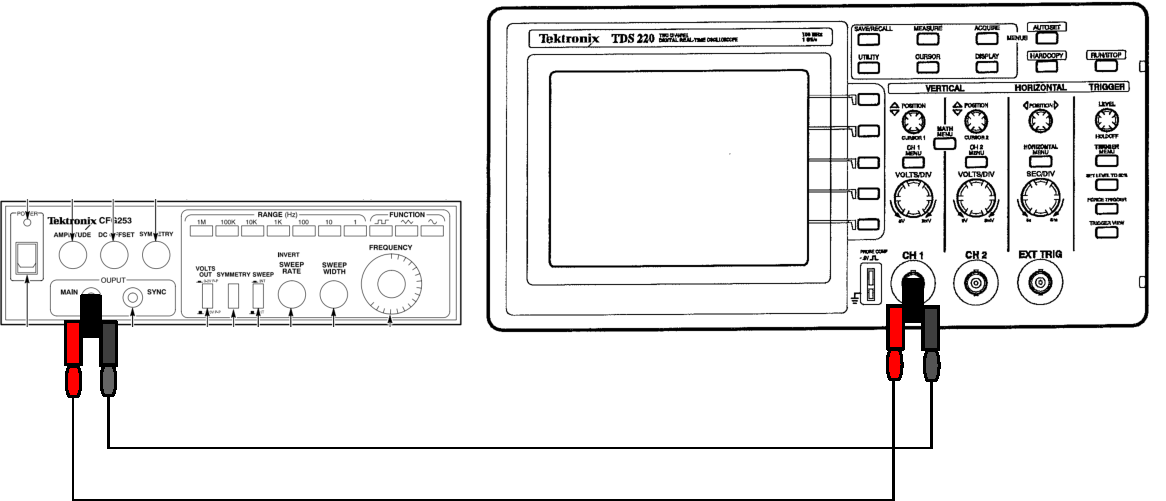
\includegraphics[width=0.9\textwidth]{./Exp9/pic/part1.pdf}
        \caption{Circuit diagram for part 1 of this experiment.}
        \label{fig:part1}
\end{figure}


\begin{enumerate}
\item Look at a 0.5 Hz sine wave on CH1 of the oscilloscope. You can set this on the function generator by selecting the 1 Hz RANGE button, and turning the frequency dial to 0.5. Set the amplitude of the wave such that it is 2 V from the bottom to the top (peak-to-peak). Set the SEC/DIV so that you can see the signal ``being drawn'' across the screen. Since the scope is more accurate at frequency counting than the function generator knob, use the horizontal scale to confirm that your sine wave is truly at 0.5 Hz. You can press RUN/STOP to freeze the image.

\item Now change the frequency of the sine wave to 10 kHz. You will need to change the horizontal scale (SEC/DIV) to something faster to see this wave. Set the trigger source to be CH1. This means that the scope is using the signal itself to figure out when to trigger. Adjust the trigger level while holding down ``TRIGGER VIEW'', and set the dashed line somewhere on the wave. Does the signal look like a standing wave?

\item What is the maximum amplitude that the function generator can produce? What is the maximum and minimum VOLTS/DIV that the oscilloscope can read? What is the minimum SEC/DIV that the scope can read? What does this tell you about the range and type of signals the scope is useful for and not useful for?

\item One measure of the performance of a device is its signal-to-noise ratio, or SNR. The signal on a sine wave can be interpreted as the peak-to-peak voltage, or twice the amplitude. The noise is the variations on that wave, or the thickness of the signal. Turn down the amplitude of the wave using the function generator until it only a few 10s of millivolts peak-to-peak. You will need to adjust the trigger level. Zoom in on your 10 kHz sine wave by decreasing the VOLTS/DIV on the oscilloscope, until you can see the noise on top of the signal, and measure its amplitude. The amplitude of noise should {\bf{not}} depend on the amplitude of the waveform. What is the signal to noise ratio of a wave with $2V$ peak-to-peak?

\end{enumerate}

\subsection{Human pulse}

Oscilloscopes allow us to analyze periodic phenomena qualitatively and quantitatively. Most sensors output some sort of voltage signal. In this part, you will use a pressure sensor to measure your pulse. You need to power the pressure sensor circuit board using 5V from the B-output of the power supply, connected to VCC and to GND. See Figure \ref{fig:part2}.

\begin{figure}[h!]
        \centering
            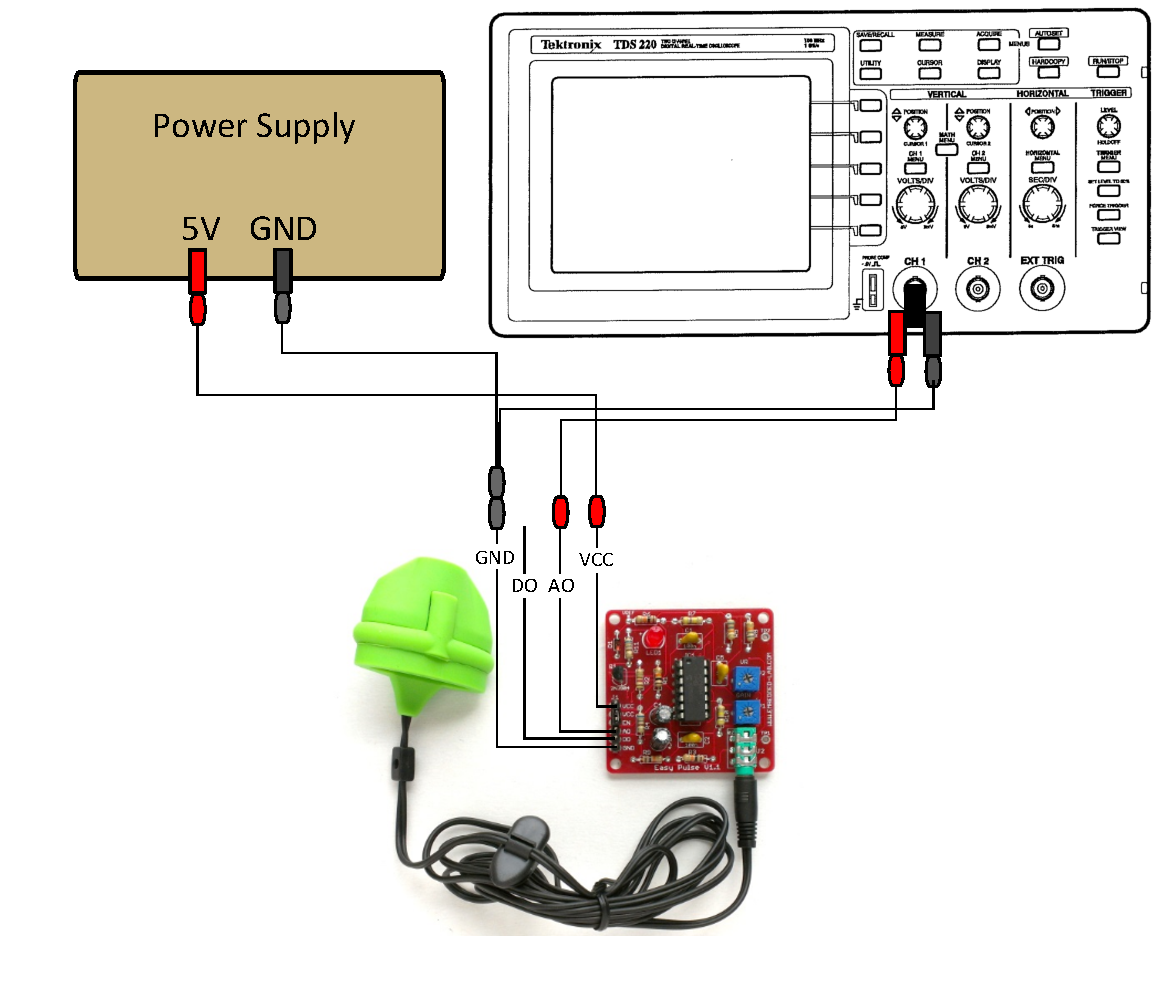
\includegraphics[width=0.9\textwidth]{./Exp9/pic/part2.pdf}
        \caption{Circuit diagram for part 2 of this experiment. Note that the Power Supply, circuit board, and oscilloscope all share the same GROUND.}
        \label{fig:part2}
\end{figure}

\begin{enumerate}
\item When examining a person's pulse, the scope can be useful for determining the frequency, amplitude, and pulse duration. Think of a couple simple experiments you can do to see how to change these properties of a human pulse. For example, you should be able to increase the frequency of the pulse by doing some jumping jacks.

\item Put the green sensor on your index finger and plug the analog signal (AO) from the circuit into the oscilloscope. Turn the horizontal knob until the sec/div is something long (~500 ms - 1 s) Measure the three quantities identified above, and try those experiments you thought of. You can ``freeze'' the image on the scope by pressing the ``Run/Stop'' button.

\item Given the structure of the pulse signal, measuring the pulse width is not well-defined. The digital output (DO) of the sensor circuit puts out a high voltage once the pressure goes above a certain level, and goes back to zero when it goes below that threshold. This results in a square wave that has better defined boundaries of where the pulse begins and ends. Measure the pulse width in this way.

\item Measure the SNR of your pulse using the method from the last experiment.
\end{enumerate}

\begin{center}
Connector Key For Pulse Circuit Board\\
\begin{tabular}{ |l | l | } \hline
  \textbf{Connector Color} & \textbf{Connector} \\ \hline
  Black & Ground \\ \hline
  Blue & DO \\ \hline
  Yellow & AO \\ \hline
  Red & VCC \\ \hline
\end{tabular}
\end{center}

\subsection{Sound waves}

As we explored in the last lab, standing sound waves can be made and amplified in certain types of resonant cavities, and the length of these cavities can tell us properties of the waves. Sound waves can also be digitized using a microphone, and then analyzed using an oscilloscope. In this part of the lab you will create and detect sound waves through electronic means, and learn more about the trigger function of the oscilloscope.

Remember that sound waves are longitudinal pressure waves, created by moving regions of alternating high and low pressure. For a speaker to make sound, an electronic voltage signal, like the ones above, are used to move a membrane forward and backwards, pushing air at set intervals to create a sound wave as described above. To detect sound waves, a microphone does exactly the opposite. A membrane is moved around by pressure waves in the air, and this motion is detected electronically, much like the pressure sensor in the pulse reader. This is similar to how your ear works!

The similarities in creating and detecting waves electronically means that we can use speakers as microphones and vice-versa. The only difference is that each tool is optimized for the function indicated by its name. A speaker makes a poor microphone, and a microphone makes a poor speaker, but the simpler these components are, the better their uses can be interchanged. Note that unfortunately, it is not possible for us to make noises with our eardrum.

\begin{figure}[h!]
        \centering
            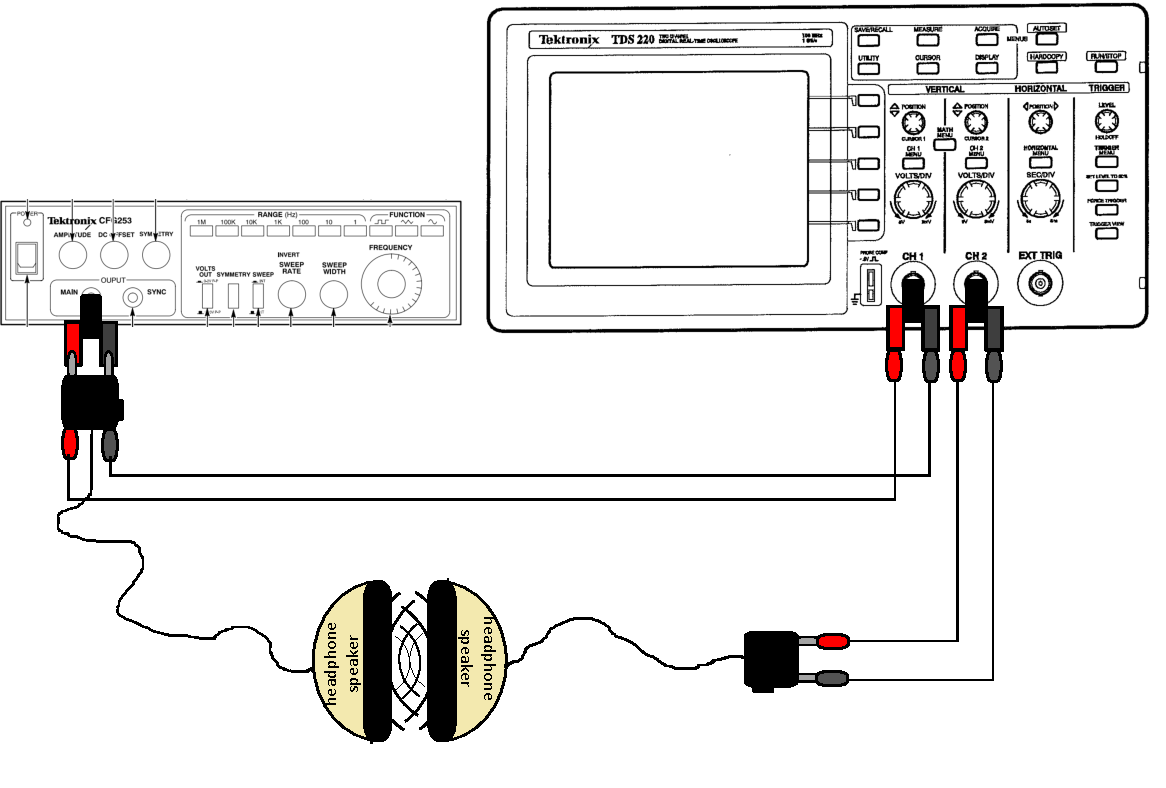
\includegraphics[width=0.7\textwidth]{./Exp9/pic/part3.pdf}
        \caption{Circuit diagram for part 3 of this experiment.}
        \label{fig:part3}
\end{figure}

\begin{enumerate}
\item To create a sound wave, hook up the output of the function generator to the headphone speaker, as partially shown in Figure \ref{fig:part3}. There is a tab on the side of the headphone adapter to tell you which pin corresponds to ground. Try a sine wave with a frequency of around 500 Hz to begin with, turn up the amplitude to a bearable level, and tune the frequency until you hear a tone you can listen to without cringing. What are the frequency limits of your hearing range? How do the triangle or square waves sound in comparison to the sine wave?

\item Also hook up this signal to CH1 on the oscilloscope so you can see what exactly you are sending to the speaker. Make sure red matches red and black matches black! We will use this signal as a trigger. So in the trigger menu, change the SOURCE to CH1, and adjust the trigger level and horizontal scale knobs until you see a synchronized wave. Try to have at least 2 divisions per period.

\item Hook up the other speaker to CH2 on the oscilloscope (Press the CH2 MENU button to have it show up on the screen), and place the headphone speaker over it so that they are facing each other. Turn up the sensitivity of the oscilloscope until you can see the detected sound wave.  You may want to strap a rubber band around both speakers to keep them together.

\item Determine the SNR of the source sound wave and the sound wave meausred through the second speaker.

\item Calculate the ratio of amplitudes of original signal and the detected signal with error. You can determine the error in the ratio by propagating uncertaines in the measured signals, interpreting the SNR as the {\it{relative uncertainty}}.

\item What is the phase of the detected wave relative to the source wave? Can you explain why?

\item Scroll around the frequency a bit and see if there are any resonances (places where the amplitude of the detected signal increases dramatically). What do these resonances mean?

\item Tune the frequency until it is out of your hearing range (higher or lower). Perhaps turn the amplitude down if you decide to go higher. Can you still see the signal? How high or low can you go before there is no detected signal? Why?

\end{enumerate}




\newpage

\section*{Scope and Function Generator Cheat Sheet}

\subsection*{Key to the oscilloscope}

\begin{figure}[h!]
        \centering
            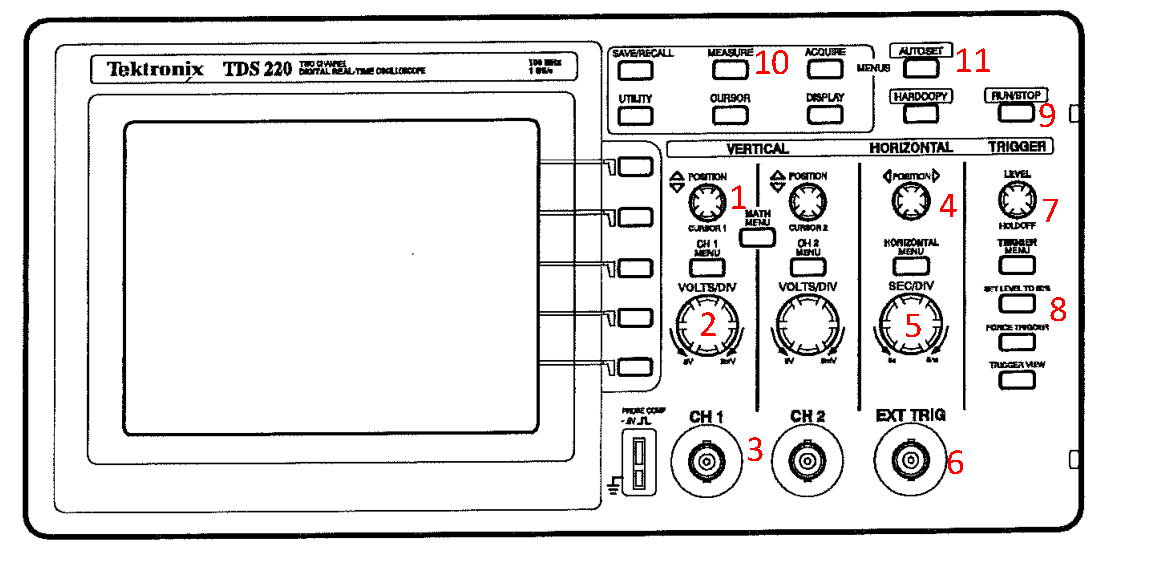
\includegraphics[width=0.9\textwidth]{./Exp9/pic/scope_label.pdf}
        \caption{Schematic of the oscilloscope you will use in this Experiment.}
        \label{fig:osc}
\end{figure}

%\subsection*{Vertical Controls}
\begin{enumerate}

%1
\item \textbf{CH1 POSITION} This knob simply adds a constant value to any point that is going to be displayed on the screen for CH1.
%2
\item \textbf{VOLTS/DIV} This knob sets the y-scale of the plot. You are changing how many volts each vertical division on the graph corresponds to. You can see the value on the bottom of the screen for each channel.
%3
\item \textbf{CH1 Input}  Where you plug in your input signal. Note that you always need to put in two wires (plus/minus), since voltage is always relative.
%4
\item \textbf{HORIZONTAL POSITION} This knob allows you to scroll left or right on the signal, which is like looking forwards or backwards in time.
%5
\item \textbf{SEC/DIV} This knob sets the x-axis scale on the screen. Each box will correspond to the number of seconds indicated on bottom of the screen.
%6
\item \textbf{EXT TRIG} This is where you plug in the trigger signal, that is, some periodic wave that you know is at the same frequency as the signal you are trying to analyze.
%7
\item \textbf{TRIGGER LEVEL} Whether you are triggering off of an external signal, or the CH1 or CH2 input signals, this knob will set where on the trigger signal we are triggering from. In other words, what part of the signal we are synching up the timing with.
%8
\item \textbf{SET TO 50\%} If you are having trouble setting the trigger level correctly, this button will automatically set it halfway between the max and min of the trigger signal. From here, you can usually adjust easily.
%9
\item \textbf{RUN/STOP} Freezes the current image on the screen.
%10
\item \textbf{MEASURE} Brings up the measure menu, from which you can access the internal measuring functions of the scope, including readings of frequencies for input signals.
%11
\item \textbf{AUTOSET} You can press this button if you are having issues getting anything to work properly. But once you do, you'll need to look through and make sure you understand what has changed.
\end{enumerate}

\subsection*{Additional notes}
\begin{enumerate}
\item You can turn on or off each channel by hitting the CH 1(or 2) MENU button a couple times. These buttons also display options for each channel, including whether you want AC or DC coupling. With this option, you can choose to couple to direct current or alternating current signals. Coupling to a signal is a another way of saying the scope is sensitive to it. Usually we will only ever need to be DC mode. AC mode is mostly for looking at noise, or periodic signals that have a large offset. For this lab, keep it in DC mode.
\end{enumerate}

\newpage

\section*{Key to the function generator}

\begin{figure}[h!]
        \centering
            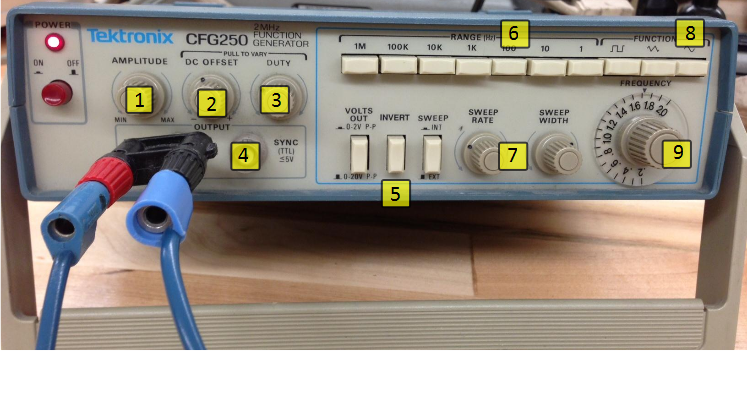
\includegraphics[width=0.9\textwidth]{./Exp9/pic/fgen.png}
        \caption{Schematic of the function generator you will use in this experiment.}
        \label{fig:gen}
\end{figure}

\begin{enumerate}
\item \textbf{Amplitude.} Adjusts the peak to peak amplitude of the outgoing wave.
\item \textbf{DC offset.} Adds a constant value to every point on the wave.
\item \textbf{Duty.} Adjusts the width of the concave part of the wave relative to the convex part. Is mostly for use with the square wave. In that case, it will make the top-bounded squares wider, and thelower bounded areas narrower.
\item \textbf{Output and Sync.} Outputs the desired function. Sync outputs the same thing but with lower amplitude.
\item \textbf{Volts Out, Invert, Sweep.} ``Volts out" sets the scale of the amplitude, ``Invert" inverts the signal, and ``Sweep" puts the device in a mode where it begins varying the frequency of the signal.
\item \textbf{Range options.} Sets the scale on the frequency knob (9)
\item \textbf{Sweep options.} Adjusts the rate and width of the range of frequencies to sweep over.
\item \textbf{Function.} Option to output square, triangle, or sine wave.
\item \textbf{Frequency dial.} Sets the frequency of the output.
\end{enumerate}
